\section*{Results}

In Figure 4 and 5: Our first successful keep-alive connection, where you can see that one thread is reused for multiple requests. %TODO: why not for all requests the same thread ?  
And a simple CGI Script where we display the environment variables REMOTE\_HOST and REMOTE\_ADDR. 

\begin{figure}[h]
    \centering
    \begin{minipage}{0.55\textwidth}
        \centering
        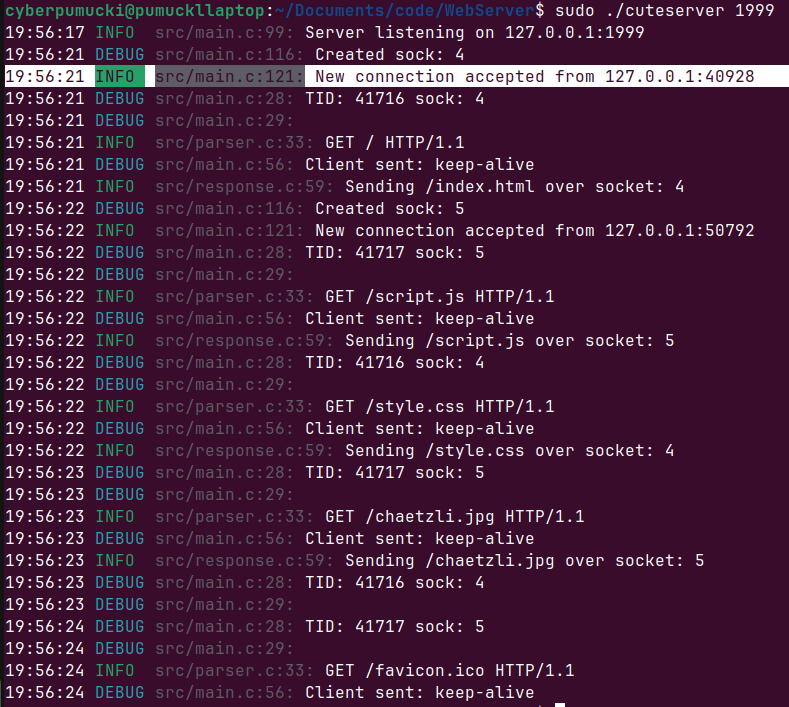
\includegraphics[width=\textwidth]{figures/keep-alive.png}
        \caption{Keep-Alive: Multiple Requests handled over one Connection}
    \end{minipage}
    \hfill
    \begin{minipage}{0.35\textwidth}
        \centering
        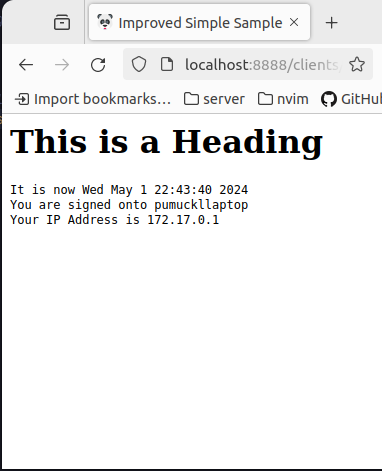
\includegraphics[width=\textwidth]{figures/cgi.png}
        \caption{First simple CGI Script with Environment Variables}
    \end{minipage}
\end{figure}
\vspace{-15pt}
\subsection*{Performance Testing}
We wanted to test the influence of the number of worker threads on the performance of our application. For this we used \textbf{Locust} \footnote{https://locust.io/} to tests POST and GET requests to our application, as well as static file requests. \\

\textbf{Static File Tests}: 
For these tests we used the following Locust Configuration: 500 users, ramp up 50 users/second, runtime 60 seconds. We tested requests to a static file (without CGI). The graphs for 2 versus 3 worker threads exhibit similar trends, so the application runs relatively stable. 
The graph shows an initial peak in response time, followed by a gradual decline and stabilization at lower values. We can only explain this result by assuming that the responses are being cached somewhere.
The Number of Requests doesn't differ enormously, but the Average Response Time for 2 Threads is 239.07ms, while with 3 Threads it's reduced by about 85ms (154.19ms). This indicates that multithreading reduces the response time per request. 

\begin{figure}[h]
    \centering
    \begin{minipage}{0.45\textwidth}
        \centering
        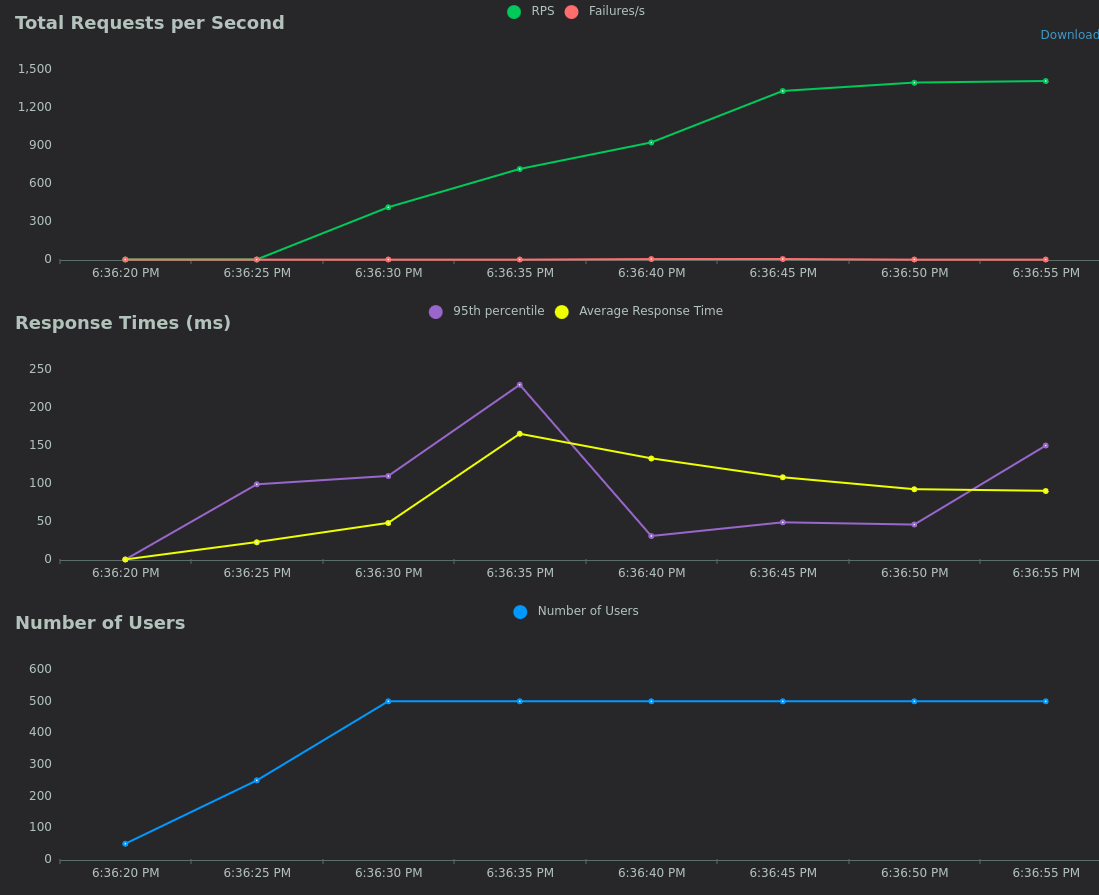
\includegraphics[width=\textwidth]{figures/2threads.png}
        % 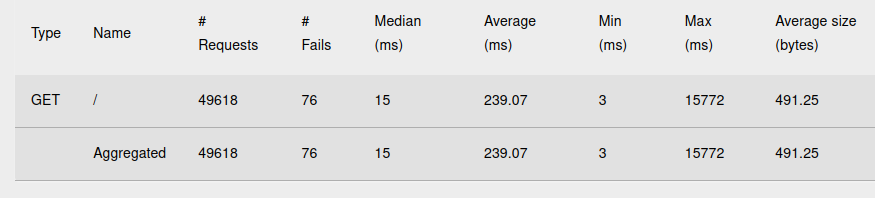
\includegraphics[width=\textwidth]{figures/2_threads_chart.png}
        \caption{Results with 2 Worker Threads}
    \end{minipage}
    \hfill
    \begin{minipage}{0.45\textwidth}
        \centering
        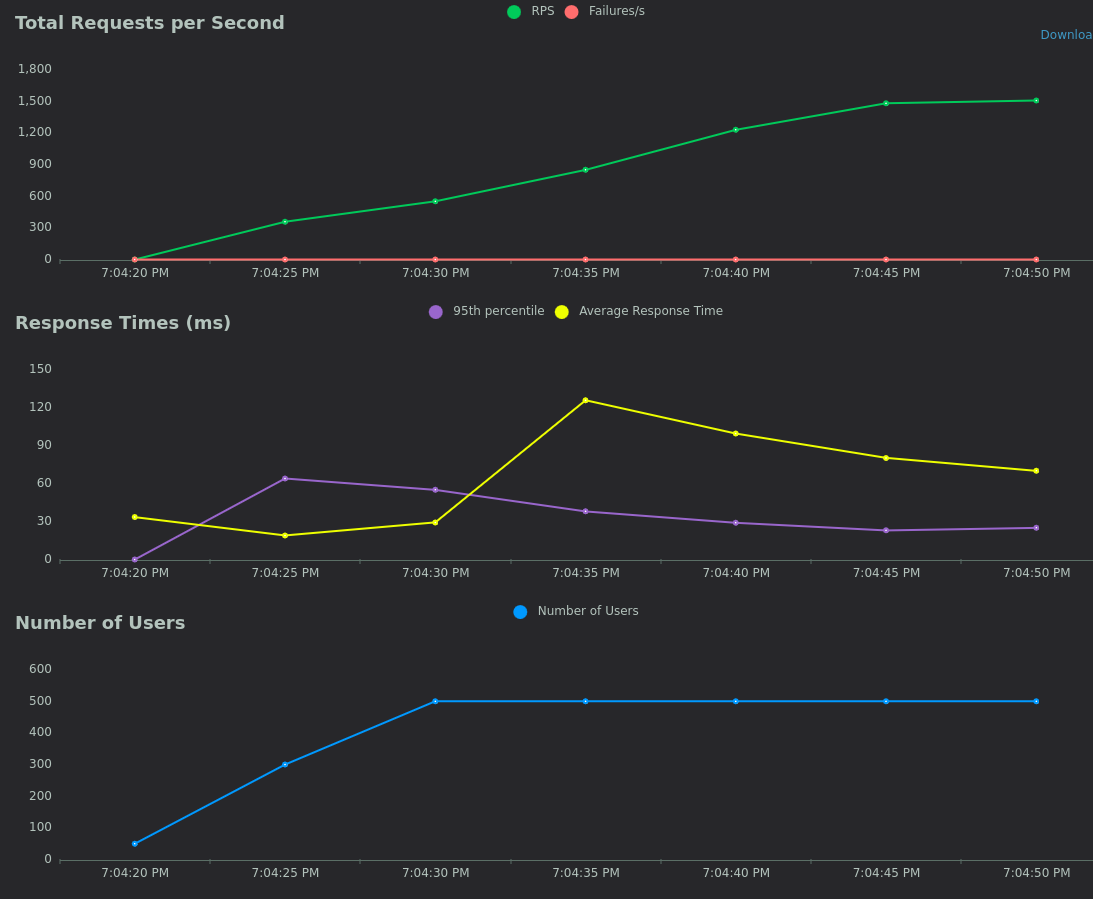
\includegraphics[width=\textwidth]{figures/3threads.png}
        % 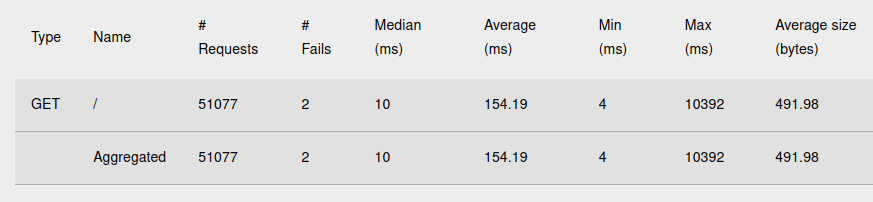
\includegraphics[width=\textwidth]{figures/3_threads_chart.png}
        \caption{Results with 3 Worker Threads}
    \end{minipage}
\end{figure}


